\documentclass[12pt]{article}
\usepackage{graphicx}
\usepackage[margin=2cm, a4paper]{geometry}
\usepackage{setspace}
\usepackage{pdfpages}
\usepackage{float}
\usepackage{amsmath}
\usepackage{fancyvrb}
\usepackage{amssymb}
\usepackage{minted}
\usepackage{enumitem}
\usepackage[colorlinks,linkcolor=blue]{hyperref}


\renewcommand{\contentsname}{Contents}
\renewcommand{\figurename}{Figure}
\renewcommand{\tablename}{Table}
\hypersetup{
    colorlinks=true,
    linkcolor=black,
    filecolor=magenta,      
    urlcolor=blue,
}
\newcommand{\mytitle}{DSDL Lab 2}
\newcommand{\myauthor}{B13902022 Richard Lai}

\usepackage{fancyhdr}
\pagestyle{fancy}
\fancyhead{}
\fancyhead[L]{\mytitle}
\fancyhead[R]{\myauthor}

\usepackage[english]{babel}
\newtheorem{theorem}{Theorem}[section]
\newtheorem{corollary}{Corollary}[theorem]
\newtheorem{lemma}[theorem]{Lemma}

\usepackage{amsthm}
\theoremstyle{definition}
\newtheorem{definition}{Definition}[section]
\theoremstyle{remark}
\newtheorem*{remark}{Remark}

\title{\mytitle}
\author{\myauthor}
\date{\today}

\begin{document}
\maketitle

\section{Part 1}
\subsection{}
\inputminted[firstline=2,lastline=37,fontsize=\small]{verilog}{lab2.v}
\subsection{}
\begin{figure}[H]
    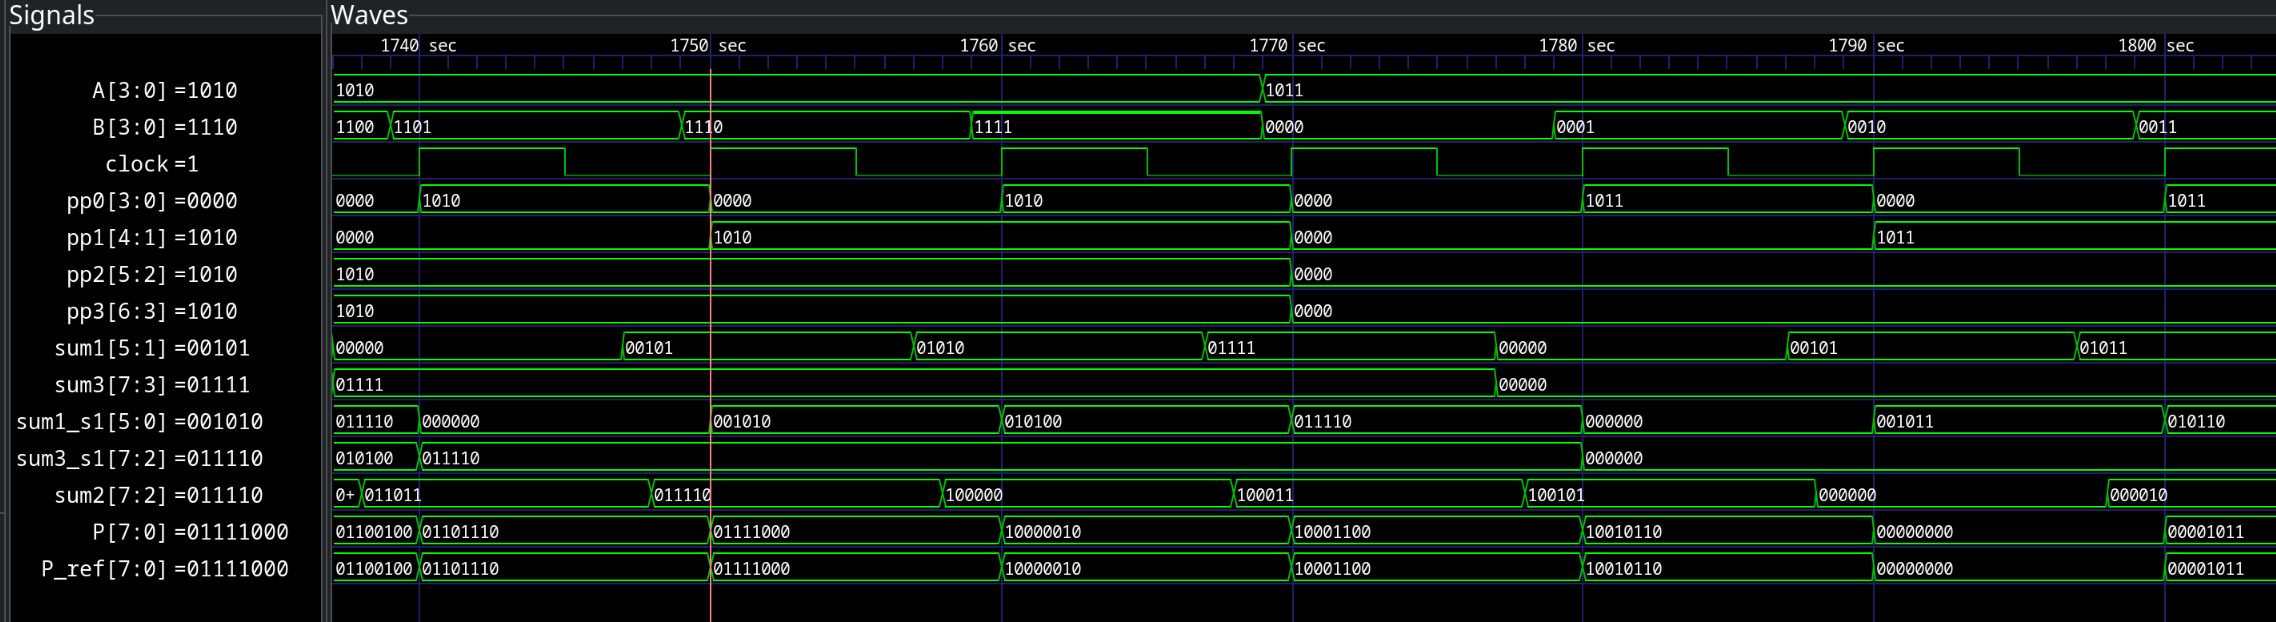
\includegraphics[width=\linewidth]{1-2.png}
\end{figure}
\subsection{}
In the worst-case scenario, data arriving just after a clock edge must wait almost a full cycle to be sampled by Stage 0, After being sampled by the input register, the data passes through two additional pipeline stages before reaching the output register. The latency is 3 clock cycles in total. Given the default testbench clock cycle of 10 ticks, the total latency is \textbf{30 ticks}.
\section{Part 2}
\subsection{}
In a pipelined architecture, the minimum clock cycle is constrained by the longest combinational delay between any two sequential registers (the critical path).  

We can look at mult\_fast: Stage 1 maximum delay is 7 ticks, and stage 2 maximum delay is 8 ticks.  

Hence, the absolute minimum clock cycle to ensure timing requirements are met without a race condition is 8 ticks.

\subsection{}
\inputminted[firstline=40,lastline=80,fontsize=\small]{verilog}{lab2.v}
\begin{figure}[H]
    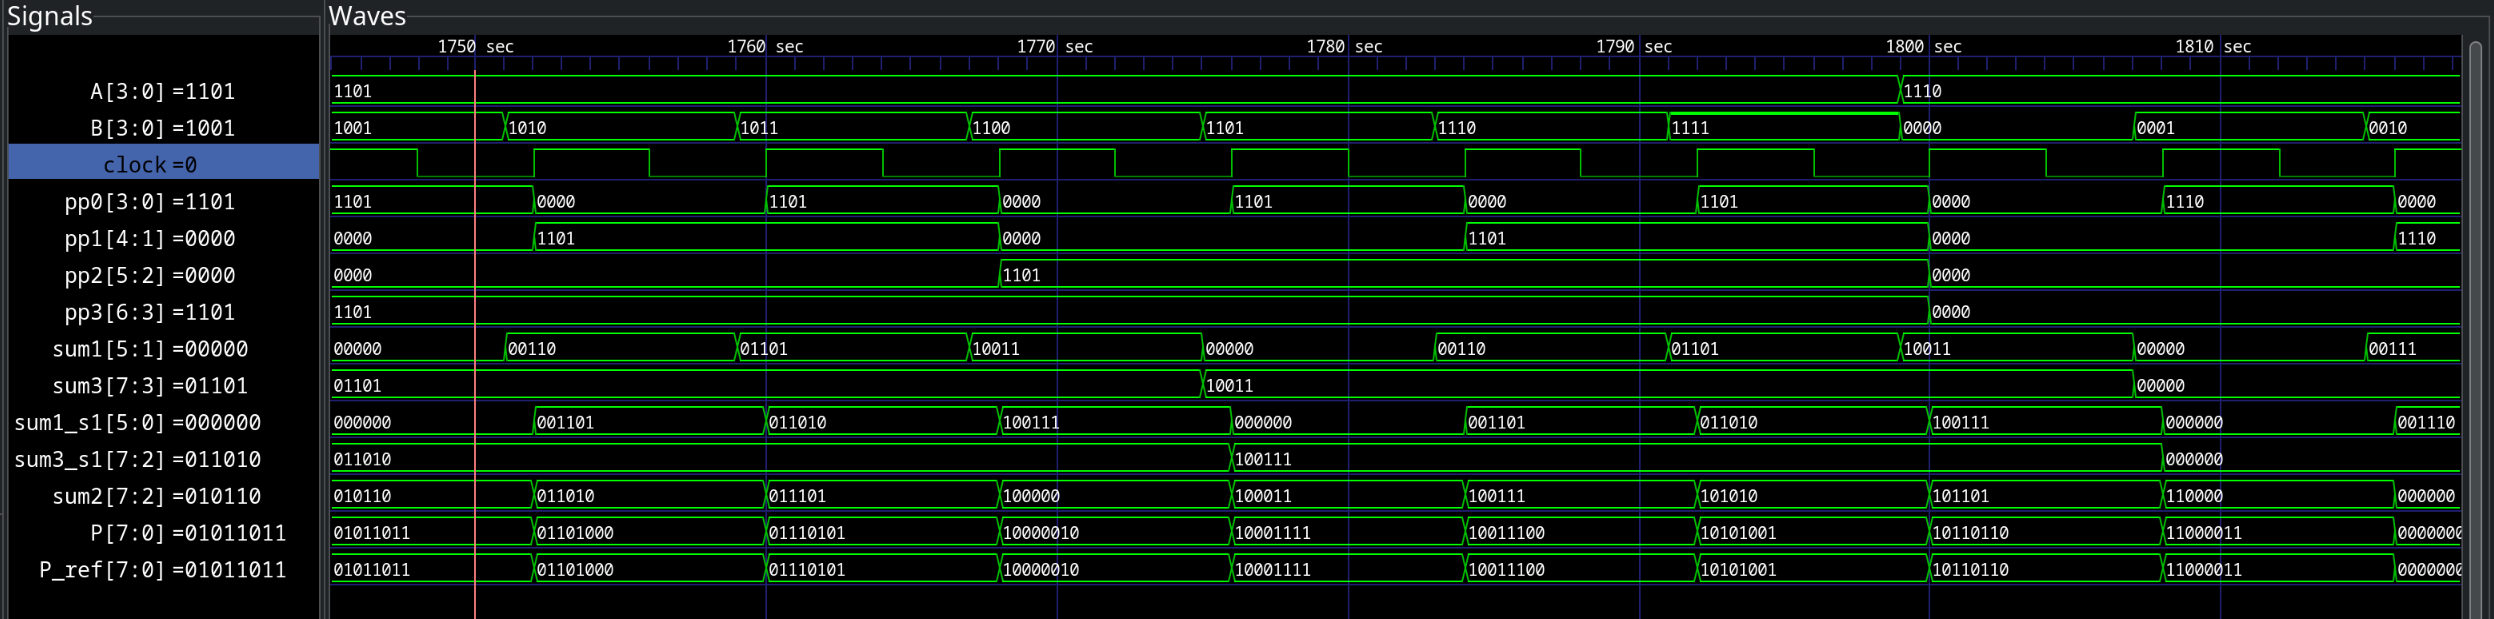
\includegraphics[width=\linewidth]{2-2.png}
\end{figure}

\end{document}
% how to display codes?
% \begin{minted}[frame=lines,framesep=2mm,baselinestretch=1.2,linenos,breaklines]{python}
% \end{minted}

% how to display images?
% \begin{figure}[H]
%     \centering
%     \includegraphics[width=0.5\linewidth]{}
%     \caption{Caption}
% \end{figure}
% test
